%\documentclass{monashthesis}                          %% Final version. Double spaced & double-sided.
\documentclass[a4paper, 11pt]{article} %% Save paper when producing drafts
%\newcommand\bmmax{8}

%\usepackage{amsmath}
%\usepackage{graphicx,psfrag,epsf,enumerate}
%\usepackage{enumerate}
%\usepackage{natbib}
%\usepackage{url} % not crucial - just used below for the URL 
%
%\usepackage{amssymb, qtree, bm, multirow, textcmds, siunitx,paralist}
%\usepackage{mathrsfs, float, booktabs,todonotes,amsthm}
%\usepackage[bb=boondox]{mathalfa}
%\usepackage{tikz}
%\usetikzlibrary{arrows,positioning,shapes,fit,calc}
%\usepackage{amsfonts}
\usepackage[a4paper,left=2.5cm,right=1.5cm,top=3cm,bottom=2.5cm]{geometry}

\usepackage{bm, amsmath, graphicx,psfrag,epsf,enumerate, paralist, amsfonts, pdfpages}
\usepackage{amssymb, qtree, multirow, textcmds, siunitx, mathrsfs, float, booktabs, isomath}
%\usepackage[bb=boondox]{mathalfa}
\usepackage{tikz}
\usetikzlibrary{arrows,positioning,shapes,fit,calc}
\usepackage[pdftex,colorlinks=true]{hyperref}
\hypersetup{citecolor=blue,linkcolor=blue,urlcolor=blue}

%\DeclareNameAlias{sortname}{last-first}
\DeclareMathOperator*{\argmin}{arg\,min}
\newcolumntype{L}{>{$}l<{$}} % math-mode version of "l" column type
\def\mathbi#1{\textit{ #1}}
\def\mathB#1{\textbf{ #1}}
\def\E{\text{E}}
\def\var{\text{Var}}
%\renewcommand{\thetable}{\Alph{chapter}\arabic{table}}
%\mathtoolsset{showonlyrefs=true}


\def\PQ{\begin{pmatrix}\bm{P}\\[-0.2cm]\bm{Q}\end{pmatrix}}
\def\bt{\begin{pmatrix}\tilde{\bm{b}}_{t+h}\\[-0.2cm]\tilde{\bm{t}}_{t+h}\end{pmatrix}}

\newtheorem{definition}{Definition}[section]

\usepackage[natbib=true,backend=bibtex,style=authoryear-comp,dashed=false,maxbibnames=99,firstinits=true,maxcitenames=3,url=true,doi=false,isbn=false]{biblatex}

\DeclareFieldFormat{url}{\url{#1}}
\DeclareFieldFormat[article]{pages}{#1}
\DeclareFieldFormat[inproceedings]{pages}{\lowercase{pp.}#1}
\DeclareFieldFormat[incollection]{pages}{\lowercase{pp.}#1}
\DeclareFieldFormat[article]{volume}{\mkbibbold{#1}}
\DeclareFieldFormat[article]{number}{\mkbibparens{#1}}
\DeclareFieldFormat[article]{title}{\MakeCapital{#1}}
\DeclareFieldFormat[article]{url}{}
\DeclareFieldFormat[book]{url}{}
\DeclareFieldFormat[inbook]{url}{}
\DeclareFieldFormat[incollection]{url}{}
\DeclareFieldFormat[inproceedings]{url}{}
\DeclareFieldFormat[inproceedings]{title}{#1}
\DeclareFieldFormat{shorthandwidth}{#1}
% No dot before number of articles
\usepackage{xpatch}
\xpatchbibmacro{volume+number+eid}{\setunit*{\adddot}}{}{}{}
% Remove In: for an article.
\renewbibmacro{in:}{%
	\ifentrytype{article}{}{%
		\printtext{\bibstring{in}\intitlepunct}}}
% Get rid of months in dates (not sure that this works)
\AtEveryBibitem{\clearfield{month}}
\AtEveryCitekey{\clearfield{month}}

\DeclareMathVersion{normal2}


\title{Probabilistic Forecasts for Hierarchical Time Series}

\bibliography{References_Pre-submission_review}

\begin{document}

\def\spacingset#1{\renewcommand{\baselinestretch}%
	{#1}\small\normalsize} \spacingset{1}

\pagenumbering{roman}


\includepdf[pages={-}]{Title-page.pdf}
%{\sf\tighttoc}


\newpage
\pagenumbering{arabic}
\setcounter{page}{1}

%
%\setcounter{section}{0}
\section{Introduction}
%\setcounter{section}{0}
%\section{Introduction}

%\section{Introduction}\label{sec:intro}

	Large collections of multiple time series often follow some aggregation structure. For example, the tourism flow of a country can be disaggregated according to a geographic hierarchy of states, zones and regions. Gross Domestic Product (GDP) of a country can be taken as another example since it is by definition the aggregation of other economic variables. To ensure aligned decision making, it is important that forecasts at the most disaggregated level add up to forecasts at more aggregated levels. This property is called ``coherence''.  On the other hand ``reconciliation'' is a process whereby incoherent forecasts are made coherent. Both of these concepts have been developed extensively for point forecasting. Generalising both of these concepts, particularly the latter, to probabilistic forecasting is a gap that we seek to address in this work.  We do that by first providing a novel geometric interpretation to coherence and reconciliation in the point forecasting case. This can easily be generalised to probabilistic forecasting allowing us to derive further results for elliptical distributions as well as provide insight into forecast evaluation via multivariate scoring rules. 
	
	Traditional approaches to ensure coherent point forecasts produce first-stage forecasts at a single level of the hierarchy. To describe these we use the hierarchy in Figure~\ref{fig:7-D_Hierarchy} where the variable labeled $Tot$ is the sum of the series $A$ and series $B$, the series $A$ is the sum of series $AA$ and series $AB$ and the series $B$ is the sum of the series $BA$ and $BB$. In the bottom-up approach \citep{Dunn1976}, forecasts are produced at the most disaggregated level (series $AA$, $AB$, $BA$ and $BB$) and then summed to recover forecasts for all higher-level series. Alternatively, in the top-down approach \citep{Gross1990}, a top-level forecast is first produced (series $Tot$) and bottom-level forecasts are recovered by disaggregating the forecast using either historical or forecasted proportions. A middle-out approach is a hybrid between these two, that for the hierarchy in Figure~\ref{fig:7-D_Hierarchy} would produce first stage forecasts for series $A$ and $B$.
	
	
	In recent years, reconciliation methods introduced by \citet{Hyndman2011} have become increasingly popular. For these methods, first stage forecasts are independently produced for all series rather than series at a single level. Since these so-called `base' forecasts are rarely coherent in practice, they are subsequently adjusted or `reconciled' to ensure coherence.  Note that we use coherence and reconciliation as distinct terms, in contrast to their at times ambiguous usage in the past. To date, reconciliation has typically been formulated as a regression problem with alternative reconciliation methods resembling different least squares estimators. These include Ordinary Least Squares {OLS} \citep{Hyndman2011}, Weighted Least Squares {WLS} \citep{AthEtAl2017}, and a Generalised Least Squares (GLS) estimator \citep{Wickramasuriya2018} named MinT since it minimises the trace of the squared error matrix. These methods have been shown to outperform traditional alternatives across a range of simulated and real-world datasets \citep{AthEtAl2009, VanErven2015a, Wickramasuriya2018} since they use the information at all levels of the hierarchy and, in some sense, hedge against the risk of model misspecification at a single level.
	
	A shortcoming of the existing literature is a focus on point forecasting despite an increased understanding over the past decade of the importance of providing a full predictive distribution for forecast uncertainty \citep[see][and references therein]{Gneiting2014}. Indeed to the best of our knowledge, the work of \citet{BenTaieb2017} and \citet{Jeon2018} are the only paper to deal with coherent probabilistic forecasts \citet{BenTaieb2017} proposed an algorithm to produce coherent probabilistic forecasts and applied it to UK electricity smart meter data. In their approach, a sample from the bottom level predictive distribution is first generated and then aggregated to obtain coherent probabilistic forecasts of the upper levels of the hierarchy. Hence this method is a bottom-up approach. They propose to first use the MinT algorithm to reconcile the means of the bottom level forecast distributions, and then a copula-based approach is employed to model the dependency structure of the hierarchy. The resulting multi-dimensional distribution is used to generating empirical forecast distributions for all bottom-level series. Thus, while \citet{BenTaieb2017} provide coherent probabilistic forecasts, they do no forecast reconciliation of the distributions. In that sense, their approach is analogous to bottom-up point forecasting rather than forecast reconciliation. 
		
	\citet{Jeon2018}, on the other hand, is the only existing study that does reconciliation in probabilistic hierarchical forecasts. This method is based on cross-validation and it also does not assume any parametric distributions for predictive densities. They have applied this method to reconcile the probabilistic forecasts for temporal hierarchies of wind power in Crete. Although they argued that this approach works for cross-sectional hierarchies as well, they have not tested this in their work.   
	
	In contrast, the main objective of this thesis is to generalise both coherence and reconciliation from point to probabilistic forecasting. To facilitate this extension, we first provide a new interpretation of the point forecast reconciliation in terms of geometry. Next, we define the coherency and reconciliation based on the probabilistic forecast. We further introduce a parametric and a non-parametric approach for probabilistic forecast reconciliation. Finally, we apply these methods to two real word applications on Australian tourism flow forecasts and Australian GDP forecasts.   
	




\begin{figure}[H]
	\begin{center}
		\leaf{AA} \leaf{AB} 
		\branch{2}{A}
		\leaf{BA} \leaf{BB}
		\branch{2}{B}
		\branch{2}{Tot}
		\qobitree
	\end{center}
	\caption{Two level hierarchical diagram}\label{fig:7-D_Hierarchy}
\end{figure}
















%Many research applications involve a large collection of time series, some of which are aggregates of others. These are called hierarchical time series. For example, tourism flow of a country can be disaggregated along a geographical hierarchy: tourism flow of states, zones, and regions. Gross Domestic Product (GDP) of country can be taken as another example for hierarchical time series since GDP is by definition the aggregation of other economic variables.   
%
%When forecasting such time series, it is important to have ``coherent'' forecasts across the hierarchy: aggregates of the forecasts at lower levels should be equal to the forecasts at the upper levels of aggregation. In other words, sums of forecasts should be equal to the forecasts of the sums.
%
%The traditional approaches to produce coherent point forecasts are the bottom-up, top-down and middle-out methods. In the bottom-up approach, forecasts of the lowest level are first generated and they are simply aggregated to forecast upper levels of the hierarchy \citep{Dunn1976}. In contrast, the top-down approach involves forecasting the most aggregated series first and then disaggregating these forecasts down the hierarchy based on the corresponding proportions of observed data \citep{Gross1990}. Many studies have discussed the relative advantages and disadvantages of bottom-up and top-down methods, and situations in which each would provide reliable forecasts \citep{Schwarzkopf1988,Kahn1998, Lapide1998,Fliedner2001}. A compromise between these two approaches is the middle-out method which entails forecasting each series of a selected middle level in the hierarchy and then forecasting upper levels by the bottom-up method and lower levels by the top-down method. 
%
%It is apparent that these three approaches use only a part of the information available when producing coherent forecasts. This might result inaccurate forecasts. For example, if the bottom level series are highly volatile or noisy, and hence challenging to forecast, then the resulting forecasts from the bottom-up approach are likely to be inaccurate.
%
%As an alternative to these traditional methods, \citet{Hyndman2011} proposed to utilize the information from all levels of the hierarchy to obtain coherent point forecasts in  a two stage process. In the first stage, the forecasts of all series are independently obtained by fitting univariate models for individual series in the hierarchy. It is very unlikely that these forecasts are coherent. Thus in the second stage, these forecasts are optimally combined through a regression model to obtain coherent forecasts. This second step is referred to as ``reconciliation'' since it takes a set of incoherent forecasts and revises them to be coherent. The approach was further improved by \citet{Wickramasuriya2018} who proposed the ``MinT'' algorithm to obtain optimally reconciled point forecasts by minimizing the mean squared coherent forecast errors. 
%
%%Traditional bottom-up, top-down and middle-out forecasting methods are not strictly reconciliation methods since they use only a part of the information from the hierarchy to produce coherent forecasts. 
%
%Previous studies on coherent point forecasting have shown that reconciliation provides better coherent forecasts than the traditional bottom-up and top-down methods \citep{Hyndman2011,VanErven2015a,Wickramasuriya2018}. However, this idea has not been explored in the context of probabilistic forecasting. 
%
%Point forecasts are limited because they provide no indication of forecast uncertainty. Providing prediction intervals helps, but a richer description of forecast uncertainty is obtained by estimating the entire forecast distribution. These are often called ``probabilistic forecasts'' \citep{Gneiting2014}. For example, \citet{McSharry2005} produced probabilistic forecasts for electricity demand, \citet{BenTaieb2017} for smart meter data, \citet{Pinson2009} for wind power generation, and \citet{Gel2004}, \citet{Gneiting2005a} and \citet{Gneiting2005} for various weather variables.
%
%Although there is a rich and growing literature on producing coherent point forecasts of hierarchical time series, little  attention has been given to coherent probabilistic forecasts. The only relevant papers we are aware of is \citet{BenTaieb2017} and \citet(Jeon2018). \citet{BenTaieb2017} proposed an algorithm to produce coherent probabilistic forecasts and applied it to UK electricity smart meter data. In their approach, a sample from the bottom level predictive distribution is first generated, and then aggregated to obtain coherent probabilistic forecasts of the upper levels of the hierarchy. Hence this method is a bottom-up approach. They propose to first use the MinT algorithm to reconcile the means of the bottom level forecast distributions, and then a copula-based approach is employed to model the dependency structure of the hierarchy. The resulting multi-dimensional distribution is used to generating empirical forecast distributions for all bottom-level series. Thus, while \citet{BenTaieb2017} provide coherent probabilistic forecasts, they do no forecast reconciliation of the distributions. In that sense, their approach is analogous to bottom-up point forecasting rather than forecast reconciliation. 
%
%\cite{Jeon2018} on the other hand is the only existing study that does reconciliation in probabilistic hierarchical forecasts. This method is based on cross-validation and it also does not assume any parametric distributions for predictive densities. They have applied this method to reconcile the probabilistic forecasts for temporal hierarchies of wind power in Crete. Although they argued that this approach works for cross-sectional hierarchies as well, they have not tested this in their work.    
%
%
%
%
%
%
%
%After introducing our notation in Section \ref{sec:notation}, we define what is meant by probabilistic forecast reconciliation for hierarchical time series in Section \ref{sec:definitions}. First, we provide a new definition for coherency of point forecasts, and the reconciliation of a set of incoherent point forecasts, using  concepts related to vector spaces and measure theory. Based on these, we provide a rigorous definition for probabilistic forecast reconciliation, and how we can reconcile the incoherent forecast densities in practice. 
%
%Further, due to the aggregation structure of the hierarchy, the probability distribution is degenerate and hence the forecast distribution should also be degenerate. In Section \ref{sec:reconciliation}, we discuss in detail how this degeneracy will be taken care of in probabilistic forecast reconciliation, and in Section \ref{sec:evaluation} we consider the evaluation of probabilistic hierarchical forecasts. 
%
%Some theoretical results on probabilistic forecast reconciliation in the Gaussian framework are given in Section \ref{sec:gaussian}, including a simulation study to show the importance of reconciliation in the probabilistic framework. 
%
%We conclude with some thoughts on extensions and limitations in Section \ref{sec:conclusions}.





\section{Overview of the Thesis}
%\section*{Overview of the thesis}
Forecasting hierarchical time series has been of great interest in many applications. In hierarchical time series, it is important to have ``coherent'' forecasts across the hierarchy. That is aggregates of the forecasts at lower levels should be equal to the forecasts at the upper levels of aggregation. While there is a rich literature on coherent hierarchical point forecasting, this research focuses on a probabilistic framework for coherent hierarchical forecasts through reconciliation. Structure of the research can be outlined as follows.    

\subsection*{Chapter 1: Introduction}
\begin{itemize}
	\item Background and motivation to the study
	\item Objectives
	\item Outline of the succeeding chapters
\end{itemize}

\subsection*{Chapter 2: Literature review}
  	
  	This chapter contains a thorough literature review of existing hierarchical point forecasting methods. Further, we discuss the importance of probabilistic framework in time series. Also, this chapter will review existing scoring rules for evaluating multivariate probabilistic forecasts in time series. 
  	
%  	We are planning to include this in a book chapter series in "Advanced Studies in Theoretical and Applied Econometrics".
  

\subsection*{Chapter 3: Hierarchical Forecast reconciliation}

To facilitate the extension of point forecast reconciliation to probabilistic forecasting framework, we first provide a geometric interpretation of existing point reconciliation methods, re-framing them in terms of projections. In addition to being highly intuitive, this allows us to establish a number of theoretical results. We prove two new theorems about point forecast reconciliation, the first showing that reconciliation via projections preserves the unbiasedness of base forecasts, while the second shows that reconciled forecasts dominate unreconciled forecasts via the distance reducing property of projections. 

Further, this chapter discusses bias adjustments in incoherent forecasts. The projections preserve unbiasedness in reconciled forecasts only if the incoherent forecasts are unbiased. However, in this chapter, we show that projections still be used to reconcile biased incoherent forecasts after some bias adjustments. This will also produce unbiased coherent forecasts. We carry out an application on Australian prison data to show these conceptual things in this chapter. 

We are planning to submit the work on this chapter to the International Journal of Forecasting. 



\subsection*{Chapter 4: Probabilistic forecasts for hierarchical time series}
\subsubsection*{Section 4.1}
This chapter mainly focuses on probabilistic forecast reconciliation. We provide definitions of coherence and forecast reconciliation in the probabilistic setting and describe how these definitions lead to a reconciliation procedure that merely involves a change of basis and marginalisation. We show that probabilistic reconciliation via linear transformations can recover the true predictive distribution as long as the latter is in the elliptical class. We provide conditions for which this linear transformation is a projection, and although this projection cannot be feasibly estimated in practice, we provide a heuristic argument in favour of MinT reconciliation.

This chapter also covers the topic of forecast evaluation of probabilistic forecasts via scoring rules. In particular, we prove that for a coherent data generating process, the log score is not proper with respect to incoherent forecasts. Therefore we recommend the use of the energy score or variogram score for comparing reconciled to unreconciled forecasts. Two or more reconciled forecasts can be compared using log score, energy score or variogram score, although we show that comparisons should be made on the full hierarchy for the latter two scores.

\subsubsection*{Section 4.2}
The second half of this chapter introduces a novel non-parametric framework to reconcile probabilistic forecasts. This involves producing future paths of the hierarchy by implicitly modeling the dependency structure of the hierarchy via bootstrapped training errors. Then these future paths will be reconciled to obtain coherent probabilistic forecasts. This method will be further evaluated via an extensive simulation study. A comprehensive explanation of this section is attached as the supplementary material to the paper I'm presenting in the pre-submission seminar. 

\subsubsection*{Section 4.3}
In the third section of this chapter, we apply both parametric and non-parametric probabilistic forecast reconciliation methods discussed in the previous section on producing coherent forecasts of Australian domestic tourism floor.   

We are planning to submit the work on this chapter to the Journal of Computational Statistics and Data Analysis. 






\subsection*{Chapter 5: Hierarchical forecasting on macroeconomic variables - An application to Australian GDP forecasts}

GDP of any country calculated as the aggregation of other economic variables. Thus by definition, this forms hierarchical time series. Hence in this chapter, we apply the point and probabilistic forecast reconciliation methods to forecast the Australian GDP. The results show that reconciliation improves the forecast performance in both point as well as probabilistic frameworks. 

This chapter was submitted as a book chapter series in "Advanced Studies in Theoretical and Applied Econometrics" and it is now under review. The work on this chapter will be mainly presented in the pre-submission seminar.  


\subsection*{Chapter 6: Conclusions}

The final chapter of my thesis will consist of the concluding remarks of the whole thesis and possible future extensions.  

\subsection*{Note:} 
According to the initial plan of my thesis, the first project consisted of the new definitions for point and probabilistic forecast reconciliation followed by the parametric approach. Following the feedback we received from the editors of the journal we submitted this paper, we decided to split this paper and have the first paper completely on point forecast reconciliation including some additional work on bias adjustment of point forecasts and an application to Australian prison data. All this work contains in the current working paper "Geometric View on Hierarchical Forecast Reconciliation" and this will be included as the third chapter of my thesis.

All definitions about probabilistic forecasts followed by the parametric approach are now included in the first half of the second project (Chapter 4 in my thesis) and the working paper on this is "Probabilistic Forecasts for Hierarchical Time Series"

\pagebreak
\section{Time plan for the thesis completion}


\subsection*{June 2019 - July 2019}

\begin{itemize}
	\item Finishing the analysis of Australian prison data
	\item Completing the write-up of chapter 3
	\item Expecting to submit to IJF
\end{itemize}


\subsection*{July 2019 - August 2019}

\begin{itemize}
	\item Completing the write-up of chapter 4
	\item Expecting to submit to JBES
\end{itemize}


\subsection*{August 2019 - October 2019}

\begin{itemize}
	\item Completing the Introduction, Background review and Conclusion chapters and submit the thesis
\end{itemize}


\begin{table}[h]
	\caption{Time-line for the completion}
	
		\centering 
\resizebox{\linewidth}{!}{
	\begin{tabular}{lllll }
		
		&\textbf{Thesis Chapter}& \textbf{Task description} & \textbf{Time duration} &  \textbf{Progress}\\  
		\toprule
		& & &  & \\
		1 and 2. & Introduction and Background Review &Writing the chapter.&September/2019 - October/2019 & 40\% Completed\\
		&&&&\\
		\midrule
		& & & & \\
		3. & Hierarchical forecast &  &&\\  
		& reconciliation & Completing the paper. & May/2019 - July/2019 & 75\% Completed \\
		
		&&&&\\
		\midrule
		&&&&\\
		4. & Probabilistic forecast &  &&\\  
		& reconciliation for & Completing the paper. & June/2019 - August/2019 & 90\% Completed \\
		& hierarchical time series &&&\\
		&&&&\\
		\midrule
		&&&&\\
		5. & Application & Forecasting Australian GDP & & 100\% Completed\\
		&&&&\\
		
		\bottomrule
	\end{tabular}
}
\end{table}


%\begin{table}
%	\caption{Time plan of the Research}
%	
%	\centering \small
%	\begin{tabular}{llll }
%		
%		\textbf{Thesis Chapter}& \textbf{Task description} & \textbf{Time duration} &  \textbf{Progress}\\  
%		\toprule
%		Introduction and & Understanding the problem&  & \\
%		Literature Review&and review on literature&Feb/2016 - Nov/2016&Completed\\
%		& associate with the problem.&&\\
%		& Writting the chapters. & May/2018 - July/2018 & Incomplete\\
%		\midrule
%		& Defining Coherent & & \\
%		& forecasts.  & Mar/2017 - June/2017 & Completed \\
%		Probabilistic forecast & Defining probabilistic &&\\  
%		reconciliation in the   & forecast reconciliation. & Mar/2017 - June/2017 & Completed \\
%		
%		hierarchical time series& Gaussian forecast& & \\
%		& reconciliation. &Nov/2016 - Feb/2017 & Completed \\ 
%		& Simulation study.  & Feb/2017 - June/2017 & Completed \\
%		\midrule
%		
%		Probabilistic forecast 	& Methodology 			& Nov/2016 - Feb/2017  & Completed\\  
%		reconciliation in the   & Simulation study 		& Mar/2017 - June/2017 & Completed \\
%		non-parametric framework& Providing theoretical & 					   &\\
%		&foundation				& Apr/2018 - July/2018 & Incomplete\\
%		\midrule
%		
%		& Forecasting Australian 	& 					  &\\
%		Application & Domestic Tourism Flow  	& Dec/2017 - Mar/2017 & Complete\\
%		& Forecasting Walmart sales & Oct/2017 - Mar/2019 & Incomplete\\
%		
%		
%		\bottomrule
%	\end{tabular}
%\end{table}

\mathversion{normal2}
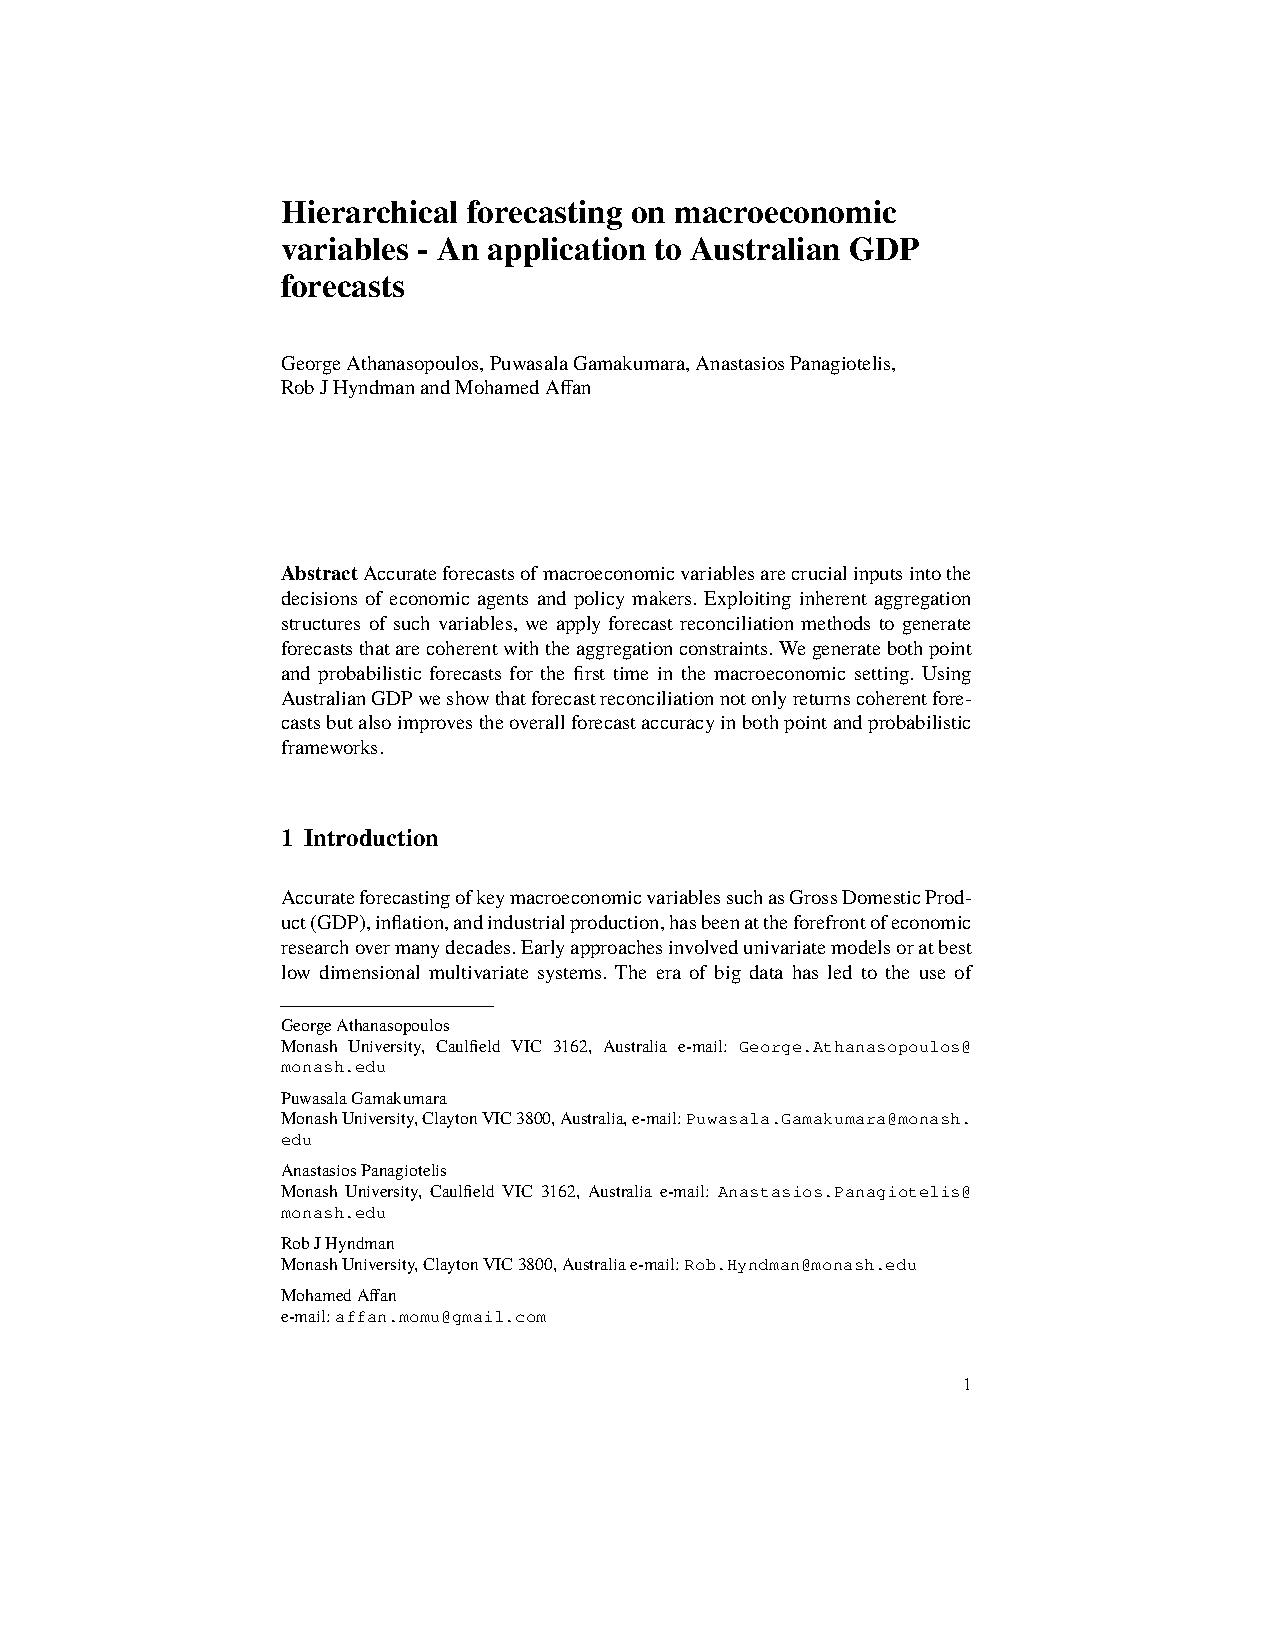
\includepdf[pages={-}]{Hierarchical_forecasting.pdf}

%\newpage
%
\section*{Supplementary materials}
\section{A non-parametric bootstrap approach for probabilistic forecast reconciliation}\label{sec:non-para}

The second half of the fourth chapter of my thesis introduces a novel non-parametric approach to reconcile hierarchical probabilistic forecasts. In this section, I provide a detailed explanation of this methodology followed by a comprehensive simulation study.

%\begin{figure}[H]
%	\begin{center}
%		\leaf{AA} \leaf{AB} 
%		\branch{2}{A}
%		\leaf{BA} \leaf{BB}
%		\branch{2}{B}
%		\branch{2}{Tot}
%		\qobitree
%	\end{center}
%	\caption{Two level hierarchical diagram}\label{fig:7-D_Hierarchy}
%\end{figure}

The proposed method initially involves obtaining probabilistic forecasts without considering the aggregation constraints. That is we first get the incoherent probabilistic forecasts. Then we reconcile these to obtain the coherent probabilistic forecasts of the hierarchy. 

\subsection{Incoherent probabilistic forecasts} \label{Subsec:Incoherent_samplePaths}
We now explain the process of obtaining incoherent sample paths. First we fit appropriate univariate models for each series in the hierarchy based on the training data $\bm{y}_{1:T}$. Then we compute 1-step-ahead training errors as $e_{i,t} = y_{i,t} - \hat{y}_{i,t}$ for $i=1,...,n$ and $t = 1,...,T$ where $\hat{y}_{i,t} = E(y_{i,t}|y_{i,1:t-1})$. These training errors will be then stored in a matrix $\bm{\Gamma}_{(T \times n)} = (\bm{e}_1,...,\bm{e}_T)'$ where $\bm{e}_t = (e_{1,t},...,e_{n,t})$ stored in the same order as $\bm{\hat{y}}_t$ for $t=1,...,T$. Next we block bootstrap a sample of size $H$ from $\bm{\Gamma}$. That is, we randomly select consecutive $H$ rows from $\bm{\Gamma}$ and store in a matrix $\bm{\Gamma}^b_{(H \times n)} = (\bm{e}^b_1,...,\bm{e}^b_H)'$ and repeat this for $b = 1,...,B$.  

Finally, we generate the $h$-step-ahead future paths using the fitted univariate models conditioning on the past observations. We incorporate bootstrapped training errors as the error series for generating future paths. This will implicitly model the contemporaneous correlation structure of the hierarchy. Further, the consecutive (block) training errors will model the serial correlation of each series. To explain this process more explicitly consider the following example. \\

\noindent
\textbf{Example 1}
Suppose we have fitted an $ARMA(p,q)$ model for the $i^\text{th}$ series of the hierarchy by using data $y_{i,1}:y_{i,T}$. i.e.
\begin{align*}
y_{i,t} &= \alpha_1y_{i,t-1} + \alpha_2y_{i,t-2}+...+\alpha_py_{i,t-p} + \beta_1\epsilon_{i,t-1} + \beta_1\epsilon_{i,t-2}+...+\beta_q\epsilon_{i,t-q} + \epsilon_{i,t},\\
y_{i,t} &= (\alpha_1 + \alpha_2L+...+\alpha_pL^{p-1})y_{i,t-1} + (\beta_1 + \beta_1L+...+\beta_qL^{q-1})\epsilon_{i,t-1} + \epsilon_{i,t},
\end{align*}
where $L$ is the well known lag or backshift operator. Then the $h$-step-ahead $b^\text{th}$ future path for $i^\text{th}$ series can be produced as,

\begin{align*}
\hat{y}^b_{i,T+h} &= (\hat{\alpha}_1 + \hat{\alpha}_2L +...+ \hat{\alpha}_pL^{p-1})y_{i,T+h-1} + (\hat{\beta}_1 + \hat{\beta}_1L+...+\hat{\beta}_qL^{q-1})\epsilon_{i,T+h-1} + e^b_{i,h}.
\end{align*}
where, $e^b_{i,h}$ is the $(h\times i)^\text{th}$ element from $\bm{\Gamma}^b$,
\begin{equation*}
y_{i,T+h-1} =
\begin{cases}
y_{i,1}:y_{i,T}       & \quad \text{for } T+h-1 \le T\\
\hat{y}^b_{i,T+1}:\hat{y}^b_{i,T+h-1}  & \quad \text{for } T+h-1 > T
\end{cases}
\end{equation*}
and 

\begin{equation*}
\epsilon_{i,T+h-1} =
\begin{cases}
\epsilon_{i,1}:\epsilon_{i,T}       & \quad \text{for } T+h-1 \le T\\
e^b_{i,1}:e^b_{i,h-1}  & \quad \text{for } T+h-1 > T
\end{cases}.
\end{equation*}

Once we get the $h$-step-ahead sample path for all $n$ series in the hierarchy, we stack them in the same order as $\bm{y}_t$. Repeating the same process for $b = 1,...,B$ we will get a set of bootstrapped $h$-step-ahead future paths of size $B$. We denote this as $\hat{\bm{\Upsilon}}_{T+h} = (\hat{\bm{y}}^1_{T+h},...,\hat{\bm{y}}^B_{T+h})'$ where each row of $\hat{\bm{\Upsilon}}_{T+h}$ represent the $h$-step-ahead sample paths for a single series and columns represent that for corresponding series of the hierarchy.  

We note that $\hat{\bm{\Upsilon}}_{T+h}$ is an empirical sample from the incoherent probability distribution of the hierarchy. However, it is very unlikely that $\hat{\bm{\Upsilon}}_{T+h}$ lies in the coherent subspace. Thus it requires the reconciliation which will be discussed in the next subsection. 

\subsection{Reconciliation of incoherent future paths}

To reconcile the incoherent sample paths, we follow the definition of reconciliation. We project each sample path in $\hat{\bm{\Upsilon}}_{T+h}$ to the coherent subspace via the projection $\bm{SG}$. i.e. for any $\bm{G}$ we can write, 
\begin{equation} \label{eq:sampleRecon_1}
\tilde{\bm{y}}_{T+h}^b = \bm{SG}\hat{\bm{y}}_{T+h}^b,
\end{equation} 
consequently we have, 
\begin{equation} \label{eq:sampleRecon_2}
\tilde{\bm{\Upsilon}}_{T+h} = \bm{SG}\hat{\bm{\Upsilon}}'_{T+h},
\end{equation} 
where, each row in $\tilde{\bm{\Upsilon}}'_{T+h}$ represent a single reconciled sample path. Further $\tilde{\bm{\Upsilon}}'_{T+h}$ form an empirical sample from the reconciled forecast distribution of the hierarchy. Any $\bm{G}$ matrix introduced in point forecast reconciliation can also be used for this sample path reconciliation. However, in the following subsection we discuss a method to find $\bm{G}$ that is optimal for probabilistic forecasts. 

\subsection{Optimal reconciliation of incoherent future paths}\label{subsec:Optimal_recon}
  
Let us now propose to find an optimal $\bm{G}$ for reconciling future paths by minimising a proper multivariate scoring rule. The respective objective function can be written as, 

\begin{equation} \label{eq:Obj_func_1}
\operatornamewithlimits{argmin}_{\bm{G}_h} \quad \E_{\bm{Q}}[S(\bm{SG}_h\hat{\bm{\Upsilon}}'_{T+h}, \bm{y}_{T+h})],
\end{equation}
where $S$ is a proper scoring rule that follows 
\begin{equation}\label{eq:prop_score}
\E_{\bm{Q}}[S(Q,\omega)] \le \E_{\bm{Q}}[S(P,\omega)] ,
\end{equation}
where $\E_{Q}[S(P,\omega)]$ is the expected score under the true distribution $Q$ \citep{Gneiting2008, Gneiting2014}.

We use the subscript $h$ on $\bm{G}$ in (\ref{eq:Obj_func_1}) to emphasis distinct $\bm{G}$ matrices for different forecast horizons. The energy score given in Table (\ref{table:scoringrules}) is a proper scoring rule. Approximating the expectations in this equation through sample means we can write,

\begin{table}[!b]
	\caption{Scoring rules to evaluate multivariate forecast densities. $\breve{\bm{Y}}_{T+h}$ and $\breve{\bm{Y}}^*_{T+h}$ be two independent random vectors from the coherent forecast distribution $\breve{\bm{F}}$ with the density function $\breve{\bm{f}}(\cdot)$ at time $T+h$ and $\bm{y}_{T+h}$ is the vector of realizations. Further $\breve{Y}_{T+h,i}$ and $\breve{Y}_{T+h,j}$ are $i$th and $j$th components of the vector $\breve{\bm{Y}}_{T+h}$. Further the variogram score is given for order $p$ where, $w_{ij}$ are non-negative weights.}\label{table:scoringrules}
	\centering\small
%	\setstretch{1.3}
	\begin{tabular}{@{}lp{8.1cm}l@{}}
		\toprule
		\textbf{Scoring rule}  & \textbf{Expression} & \textbf{Reference}           \\
		\midrule
		\text{Log score}       &
		$\text{LS}(\breve{\bm{F}},\bm{y}_{T+h}) = -\log {\breve{\bm{f}}(\bm{y}_{T+h})}$ &
		\citet{Gneiting2007}  \\\\[-0.2cm]
		\text{Energy score}    &
		$\text{eS}(\breve{\bm{Y}}_{T+h},\bm{y}_{T+h}) =
		\E_{\breve{\bm{F}}}
		\|\breve{\bm{Y}}_{T+h}-\bm{y}_{T+h}\|^\alpha -$ \par\hfill
		$\frac{1}{2}\E_{\breve{\bm{F}}}\|\breve{\bm{Y}}_{T+h}-\breve{\bm{Y}}^*_{T+h}\|^\alpha$, \,\, $\alpha \in (0,2]$ &
		\citet{Gneiting2008}  \\\\[-0.2cm]
		\text{Variogram score} &
		$\text{VS}(\breve{\bm{F}}, \bm{y}_{T+h}) =
		\sum\limits_{i=1}^{n}
		\sum\limits_{j=1}^{n}
		w_{ij}\Big(|y_{T+h,i} - y_{T+h,j}|^p -$ \par\hfill
		$\E_{\breve{\bm{F}}}|\breve{Y}_{T+h,i}-\breve{Y}_{T+h,j}|^p\Big)^2$     &
		\citet{SCHEUERER2015} \\
		\bottomrule
	\end{tabular}
\end{table}



\begin{equation}\label{eq:ES_with_Samplespaths}
\text{ES}(\bm{SG}_h\hat{\bm{\Upsilon}}'_{T+h}, \bm{y}_{T+h}) \approx \frac{1}{B}\sum_{b=1}^{B}||\bm{SG}_h\hat{\bm{y}}_{T+h,j}^b -\bm{y}_{T+h}||-\frac{1}{2(B-1)}\sum_{b=1}^{B-1}||\bm{SG}_h(\hat{\bm{y}}_{T+h,j}^b -\hat{\bm{y}}_{T+h,j}^{b+1})||.
\end{equation}
where $B$ is the empirical sample size from the coherent forecast distribution. Now we can rewrite the objective function in (\ref{eq:Obj_func_1}) as,

\begin{equation}\label{eq:Obj_func_2}
\operatornamewithlimits{argmin}_{\bm{G}} \frac{1}{N}\sum_{j=1}^{N}\left\{\frac{1}{B}\sum_{b=1}^{B}||\bm{SG}_h\bm{y}_{T+h,j}^b -\bm{y}_{T+h,j}||-\frac{1}{2(B-1)}\sum_{b=1}^{B-1}||\bm{SG}_h(\bm{y}_{T+h,j}^b -\bm{y}_{T+h,j}^{b+1})||\right\}
\end{equation}
where, the expectation $E_{\bm{Q}}$ is approximated through the sample mean over $\{\text{ES}(\bm{SG}_h\hat{\bm{\Upsilon}}'_{T+h,1}, \bm{y}_{T+h,1}),...,\\
\text{ES}(\bm{SG}_h\hat{\bm{\Upsilon}}'_{T+h,N}, \bm{y}_{T+h,N})\}$.   
Since this is hard to solve analytically, we use a numerical optimization methods to estimate the matrix $\bm{G}_h$ that minimizes above objective function and thus obtain the optimally reconciled future paths. 

\subsubsection{Reparameterisation of G} \label{subsubsec:ReparameterisationG}

We consider different parameterisations when estimating the optimal $\bm{G}$ via above optimisation process. Let,  
\begin{equation}\label{eq:StructureofG}
\bm{G}_h = (\bm{S'W}_h\bm{S})^{-1}\bm{S'W}_h.
\end{equation}
This structure for $\bm{G}_h$ will ensure $\bm{SG}_h$ is a projection matrix and it projects each sample path onto $\mathfrak{s}$. 
\begin{itemize}
	\item[\textbf{Method 1}] Minimising the objective function in (\ref{eq:Obj_func_2}) over $\bm{W}_h$. This solves an unconstrained optimisation problem 
	\item[\textbf{Method 2}] Consider the cholesky decomposition of $\bm{W}_h$. i.e. let $\bm{W}_h = \bm{R}_h'\bm{R}_h$ where $\bm{R}_h$ is an upper triangular matrix. Thus minimising  (\ref{eq:Obj_func_2}) over $\bm{R}_h$ 
	\item[\textbf{Method 3}] Similar to Method 2, minimising (\ref{eq:Obj_func_2}) over cholesky decomposition of $\bm{W}_h$ but restricted for scaling. i.e., $\bm{W}_h=\bm{R}_h'\bm{R} \quad \text{s.t} \quad \bm{i'}\bm{W}_h\bm{i}=1$ where $\bm{i}=(1,0,..,0)'$
	\item[\textbf{Method 4}] Minimising (\ref{eq:Obj_func_2}) over $\bm{G}_h$ such that $\bm{G}_h\bm{S}=\bm{I}$. This constraint will ensure that $\bm{SG}_h$ is a projection onto $\mathfrak{s}$
	  
\end{itemize}    



\subsection{Simulation study}\label{sec:Bootsrap-sim}

We now turn our attention to comparing different reconciliation methods with optimal reconciliation in a simulation setting. 

\subsubsection{Data generating process (DGP)}
For the data generating process, we consider the hierarchy is given in Figure~\ref{fig:7-D_Hierarchy}, comprising two aggregation levels with four bottom-level series. Each bottom-level series will be generated first, and then summed to obtain the data for the upper-level series. 

Initially, the error series were generated for four bottom-level series. To impose dependency among these series, errors were generated from the Gumbel copula model with beta margins. A two dimensional Gumbel copula is given by, 
\begin{equation*}
C_\theta(u_1, u_2) = exp\{-[(-ln(u_1))^\theta + (-ln(u_2))^\theta]^{1/\theta}\}. 
\end{equation*}
We generate random variates $\{u_{AA}, u_{AB}\}$ from $C_{\theta=10}(.)$ and $\{u_{BA}, u_{BB}\}$ from $C_{\theta=8}(.)$ for series $\{AA, AB\}$ and $\{BA, BB\}$ respectively. Next we generate the quantiles from beta distributions with shape parameters $\alpha = 1$ and $\beta = 3$ correspond to $\{u_{AA}, u_{AB}, u_{BA}, u_{BB}\}$. Denote these quantiles as $\{\varepsilon_{AA}, \varepsilon_{AB}, \varepsilon_{BA}, \varepsilon_{BB}\}$. 
%These quantiles are the error series use for generating bottom-level data. 

Then $\{w_{AA,t},w_{AB,t},w_{BA,t},w_{BB,t}\}$ were generated from ARIMA$(p,d,q)$ processes, where $(p,q)$ and $d$ take integers from $\{1,2\}$ and $\{0,1\}$ respectively with equal probabilities. $\{\varepsilon_{AA}, \varepsilon_{AB}, \varepsilon_{BA}, \varepsilon_{BB}\}$ were incorporated as the errors driving these ARIMA processes. The parameters for the AR and MA components are randomly and uniformly generated from $[0.3,0.5]$ and $[0.3,0.7]$ respectively. 

In practice, hierarchical time series likely to have much noisier series at lower levels of aggregation. Following the method proposed by \citet{Wickramasuriya2018}, we replicate this feature in our simulations by generating the bottom-level series $\{y_{AA,t},y_{AB,t},y_{BA,t},y_{BB,t}\}$ as follows: 
\begin{align*}
y_{AA,t} &= w_{AA,t} + u_t - 0.5v_t,\\
y_{AB,t} &= w_{AB,t} - u_t - 0.5v_t,\\
y_{BA,t} &= w_{BA,t} + u_t + 0.5v_t,\\
y_{BB,t} &= w_{BB,t} - u_t + 0.5v_t,
\end{align*}
where $u_t \sim \mathcal{N}(0,\sigma^2_u)$ and $v_t \sim \mathcal{N}(0,\sigma^2_v)$. The aggregate series in the middle-level are given by:
\begin{align*}
y_{A,t} &= w_{AA,t} + w_{AB,t} - v_t,\\
y_{B,t} &= w_{BA,t} + w_{BB,t} + v_t,
\end{align*}
and the total series is given by
\[
  y_{Tot,t} = w_{AA,t} + w_{AB,t} + w_{BA,t} + w_{BB,t}.
\]


To ensure the disaggregate series are noisier than the aggregate series, we choose $\sigma^2_u$ and $\sigma^2_v$ such that
\[
  \var(\varepsilon_{AA,t} + \varepsilon_{AB,t} + \varepsilon_{BA,t} + \varepsilon_{BB,t})
  \le \var(\varepsilon_{AA,t}+\varepsilon_{AB,t}-v_t)
  \le \var(\varepsilon_{AA,t}+u_t-0.5v_t).
\]
Similar inequalities hold when $\varepsilon_{AA,t}$ is replaced by $\varepsilon_{AB,t}$, $\varepsilon_{BA,t}$ and $\varepsilon_{BB,t}$ in the third term.
The variance covariance matrix of $\{\varepsilon_{AA}, \varepsilon_{AB}, \varepsilon_{BA}, \varepsilon_{BB}\}$ is,
$$
\bm{\Sigma} = \begin{pmatrix}
				0.0388 & 0.0385 & 0.0010 & 0.0010\\
				0.0385 & 0.0390 & 0.0008 & 0.0008 \\
				0.0010 & 0.0008 & 0.0387 & 0.0377 \\
				0.0010 & 0.0008 & 0.0377 & 0.0381 \\
			 \end{pmatrix}.
$$
Thus we choose $\sigma^2_u = 10$ and $\sigma^2_v = 7$ to satisfy the above constraints. 

\subsubsection{Simulation set up for optimal reconciliation}

\begin{enumerate}
    \item Generate time series with $2500$ data points in each, corresponds to the hierarchy in Figure \ref{fig:7-D_Hierarchy} based on the DGP explained. 
\item Consider a rolling window of $600$ observations. We refer to it the outer rolling window. 
\begin{enumerate}[i.]
	\item Inside this outer rolling window consider an inner rolling window of $T=500$ observations. 
	\item Using inner rolling window, fit univariate ARIMA models to each series in the hierarchy.
	\item Based on these fitted models, we generate $B=1000$ of $h=3$ step-ahead incoherent future paths incorporating bootstrap errors as described in Sub section \ref{Subsec:Incoherent_samplePaths}. Thus we get $\{\hat{\bm{\Upsilon}}_{T+1,j=1}, \hat{\bm{\Upsilon}}_{T+2,j=1}, \hat{\bm{\Upsilon}}_{T+3,j=1}\}$. 
	\item Repeat step (iii) for $j=1,...,N$ where $N=100$, by rolling the inner window by one step ahead at a time. 
	\item Collect $\{\hat{\bm{\Upsilon}}_{T+h,j=1},...,\hat{\bm{\Upsilon}}_{T+h,j=100}\}$ for $h=1,...,3$ into a separate arrays of matrices. 
	\item For each forecast horizon $h$, estimate the optimal $\bm{G}_h$ that will reconcile $\{\hat{\bm{\Upsilon}}_{T+h,j=1},...,\hat{\bm{\Upsilon}}_{T+h,j=100}\}$ by minimising the average energy score as explained in Subsection \ref{subsec:Optimal_recon}. Also use different reparameterisation of $\bm{G}_h$ as explained in Subsection $\ref{subsubsec:ReparameterisationG}$. Denote this as $\bm{G}^{Opt}_h$. 
	\item Roll the inner rolling window another one step ahead and repeat step (ii) and (iii). Let these future paths denoted by $\hat{\bm{\Upsilon}}_{T+h}$ for $h=1,2,3$. 
	\item Compute $\tilde{\bm{\Upsilon}}_{T+h} = \bm{SG}_h\hat{\bm{\Upsilon}}'_{T+h}$ for $h=1,2,3$ using $\bm{G}^{Opt}_h$ as well as using other $\bm{G}$ matrices used in point forecast reconciliation.
	
\end{enumerate}

\item Repeat Step 2 for $1000$ times by rolling the outer rolling window one step ahead at each time. Collect $1000$ of these reconciled future paths, $\tilde{\bm{\Upsilon}}_{T+h}$, from different reconciliation methods for $h=1,2,3$ and evaluate the forecasting performances. 
\end{enumerate}

\subsubsection{Results and discussion}
%To assess the predictive performance of different forecasting methods, we use scoring rules given in Table \ref{table:scoringrules}. To facilitate comparisons, we report skill scores \citep{Gneiting2007}. For a given forecasting method, evaluated by a particular scoring rule, the skill score 
%gives the percentage improvement of the preferred forecasting method relative to a reference method. A negative valued skill score indicates that a method is worse than the reference method, whereas any positive value indicates that the method is superior to the reference method.
Following the simulation process explained before, the probabilistic forecasts from different reconciliation methods were generated. Energy score and variogram scores were calculated to assess the predictive performance of these forecasts. Results are presented in Table \ref{table:Non-paraSimulation}. 

Mann-Whitney test for location comparison claimed that the ES and VS for all reconciled forecasts are significantly lower than that of base/incoherent forecasts. Thus it is evident that all reconciliation methods produce coherent probabilistic forecasts with improved predictive ability than incoherent forecasts. In addition to that, MinT(Shrink) and Optimal methods are having similar prediction accuracy as there is no significant difference between the scores from these reconciliation methods. However, the optimal reconciliation required high computational cost and it will increase for larger hierarchies. Further, it requires sufficient data points for the learning process of $\bm{G}$. Thus we claim to use the MinT $\bm{G}$ for reconciling bootstrapped future paths for two reasons. Firstly it is computationally effective than the optimal method and secondly, it produces accurate probabilistic forecasts at least as good as Optimal method. 


\begin{table} 
	\caption{Energy scores (ES) and variogram scores (VS) for probabilistic forecasts from different reconciliation methods. Bottom row represent the scores for base forecasts which are not coherent. The smaller the scores, the better the forecasts are.} \label{table:Non-paraSimulation}
	\centering\tabcolsep=0.08cm\small
	\begin{tabular}{@{}lSSSSSS@{}}
		\toprule
		Reconciliation &
		\multicolumn{2}{c}{h=1} &
		\multicolumn{2}{c}{h=2} &
		\multicolumn{2}{c}{h=3} \\
		\cmidrule(lr){2-3} \cmidrule(lr){4-5} \cmidrule(lr){6-7}
		method       & {}{\text{ES}} &  {\text{VS}} & {\text{ES}} &  {\text{VS}} & {\text{ES}} &  {\text{VS}} \\
		\midrule
		Optimal(Method-1) & 5.36 & 1.21 & 5.51 & 1.27 & 5.83 & 1.38 \\
		Optimal(Method-2) & 5.37 & 1.21 & 5.53 & 1.27 & 5.83 & 1.37 \\
		Optimal(Method-3) & 5.37 & 1.21 & 5.53 & 1.27 & 5.83 & 1.37 \\
		Optimal(Method-4) & 5.38 & 1.21 & 5.54 & 1.27 & 5.83 & 1.38 \\
		MinT(Shrink) & 5.33 & 1.19 & 5.50 & 1.26 & 5.77 & 1.34 \\
		WLS          & 5.43 & 1.23 & 5.60 & 1.30 & 5.89 & 1.40 \\
		OLS          & 5.51 & 1.23 & 5.70 & 1.30 & 5.98 & 1.40 \\
		\textit{Base} & \textit{5.71} & \textit{1.28} & \textit{5.94} & \textit{1.37} & \textit{6.27} & \textit{1.49} \\
		\bottomrule
	\end{tabular}
	
\end{table}




%We generate data with a sample size of $T=501$. Univariate ARIMA models are selected for each series using the \textit{auto.arima} function in the \textit{forecast} package \citep{hyndman2017forecasting} in R \citep{Rcore}. The same package was used to fit each series independently using the first 500 observations, and evaluate 1-step ahead base (incoherent) probabilistic forecasts. These were then reconciled using different projections summarised in Table~\ref{table:2}. This process was replicated using $1000$ different data sets from the same data generating processes.

%
%Table~\ref{table:3} summarizes the forecasting performance of unreconciled, bottom-up, OLS, WLS and two MinT reconciliation methods using log score, energy score and variogram score. In all cases skill scores are calculated with the bottom-up method as reference. All log scores are evaluated on the basis of bottom-level series only, however these only differ from the log scores for the full hierarchy by a fixed constant. The cell for log score of unreconciled forecasts is left blank since the log score is not proper in this context. Overall, the MinT methods provide the best performance irrespective of the scoring rule, and all methods that reconcile using information at all levels of the forecast improve upon unreconciled forecasts. Bottom-up forecasts perform even worse than unreconciled forecasts in some cases.
%
%Tables~\ref{table:4} and~\ref{table:5} break down the forecasting performance of different reconciliation methods by considering univariate scores on each individual margin.  Tables~\ref{table:4} summarises results for the top and middle-level, Table~\ref{table:5} does the same for bottom-level. The log score and CRPS are considered, while skill scores are computed with the unreconciled forecast as a reference. When broken down in this fashion, the methods based on MinT perform best for all series and always outperform bottom-up and unreconciled forecasts.
%




\mathversion{normal}
\newpage

\printbibliography
% Appendices start here




\end{document}
